\documentclass[12pt]{article}
%packages
\usepackage{amsmath}
\usepackage{amsfonts}
\usepackage{amssymb}
\usepackage{amsthm}
\usepackage{hyperref}
\usepackage[onehalfspacing]{setspace}
\usepackage[margin = 1 in]{geometry}
\usepackage{bbm}
\usepackage{indentfirst}
\usepackage{graphicx}
\usepackage{listings}
\usepackage[svgnames]{xcolor}
\usepackage{algorithm}
\usepackage{algorithmic}
\usepackage{enumitem}
\usepackage{bbold}
\usepackage{dsfont}

%shorthands
\newcommand{\sol}{\paragraph{Solution.}}
\newcommand{\iid}{\stackrel{iid}{\sim}}
\newcommand{\convprob}{\stackrel{P}{\longrightarrow}}
\newcommand{\convdist}{\stackrel{d}{\longrightarrow}}
\newcommand{\convpmean}{\stackrel{L^p}{\longrightarrow}}
\newcommand{\convas}{\stackrel{a.s.}{\longrightarrow}}
\newcommand{\ntoinf}{\stackrel{n\rightarrow\infty}{\longrightarrow}}
\newcommand{\limntoinf}{\underset{n\rightarrow\infty}{\lim}}
\newcommand{\limtoinf}{\lim\limits_{n\to\infty}}
\newcommand{\bigbrac}[1]{\left(#1\right)}
\newcommand{\bigmbrac}[1]{\left[#1\right]}
\newcommand{\biglbrac}[1]{\left\{#1\right\}}
\newcommand{\abs}[1]{\left|#1\right|}

%styles
\renewcommand{\qedsymbol}{$\blacksquare$}
\newcommand{\e}{\mathbb E}
\renewcommand{\epsilon}{\varepsilon}
\newcommand{\p}{\mathbb P}
\newcommand{\imply}{\implies}
\newcommand{\var}{\mathrm Var}
\newcommand{\cov}{\mathrm Cov}
\theoremstyle{definition}
\newtheorem{mydef}{Definition}[section]
\newtheorem{mythm}{Theorem}[section]
\newtheorem{myexm}{Example}[section]
\newtheorem{myle}{Lemma}[section]
\newtheorem{myprop}{Proposition}[section]
\theoremstyle{remark}
\newtheorem{myre}{Remark}[section]

%Titlepage
\begin{titlepage}
\title{Synthetic Data Generation}

\author{Wentao Li}
\date{\today}
\end{titlepage}

\begin{document}
\maketitle
\section*{Data overview}
\subsubsection*{Settings}
There are 8 Settings of data in total as followings:
\begin{itemize}
	\item Setting 1: 2 sites, 500 patients each site, small variance
	\item Setting 2: 2 sites, 500 patients each site, large variance
	\item Setting 3: 10 sites, 500 patients each site, small variance
	\item Setting 4: 10 sites, 500 patients each site, large variance
	\item Setting 5: 2 sites, 30 patients each site, small variance
    \item Setting 6: 2 sites, 30 patients each site, large variance
	\item Setting 7: 10 sites, 30 patients each site, small variance
	\item Setting 8: 10 sites, 30 patients each site, large variance
\end{itemize}
\subsubsection*{Data information}
And in each data setting, data are consisted of
\begin{enumerate}
	\item 4 categorical data, value in $\{0,1\}$
	\item 6 categorical data, value in range $[-1,1.5]\in\mathbb R$
	\item 1 outcome, value in $\{0,1\}$
	\item Site ID, represents the id of which site the entry belongs to
	\item Site sample size, represents the number of samples in this specific setting
	\item Log-odds ratio for each sample
	\item Number of true positive, true negative, false positive, false positive, false negative
\end{enumerate}
\subsubsection*{Screenshot}
\begin{figure*}[h!]
	\centering
	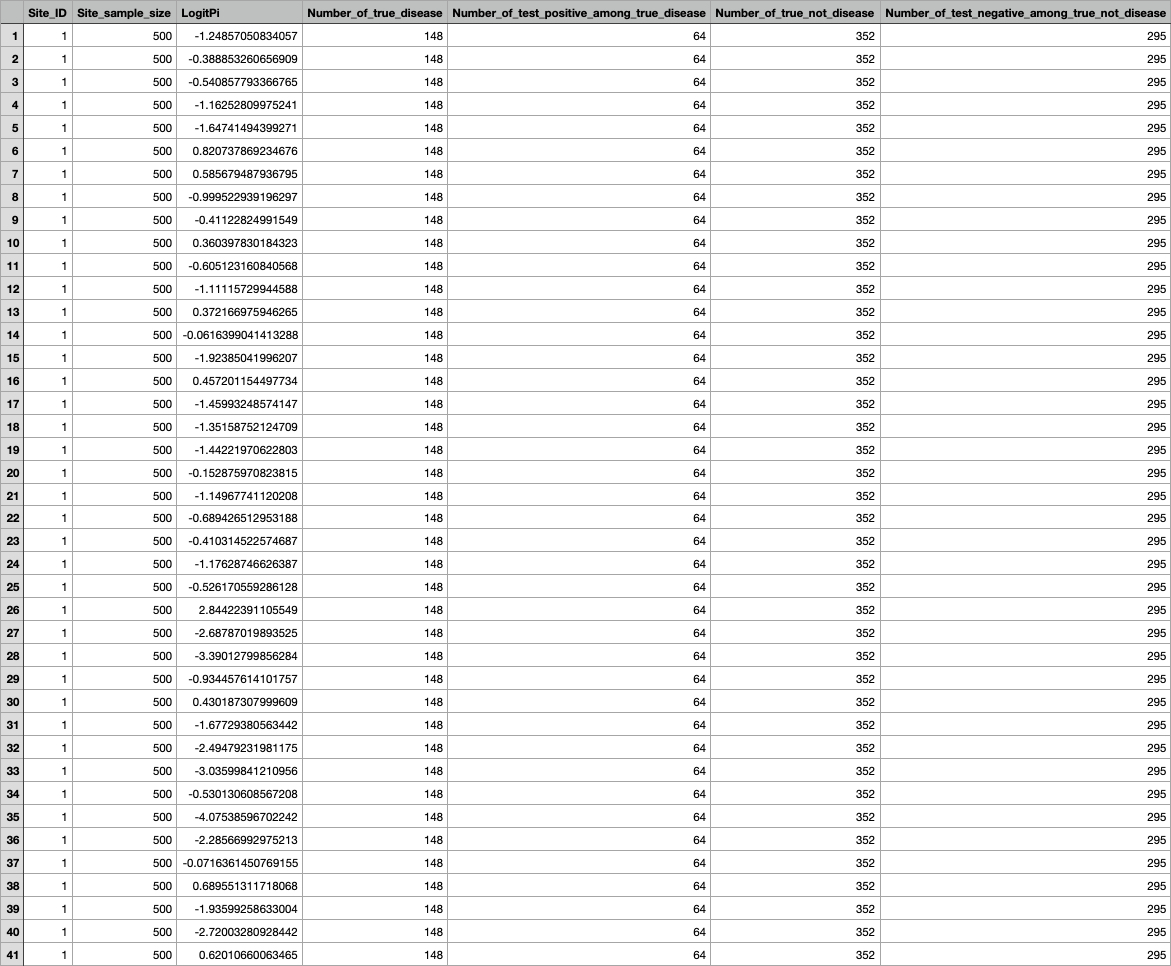
\includegraphics[scale=0.4]{data_screenshot_2.jpg}
\end{figure*}
\begin{figure*}[h!]
	\centering
	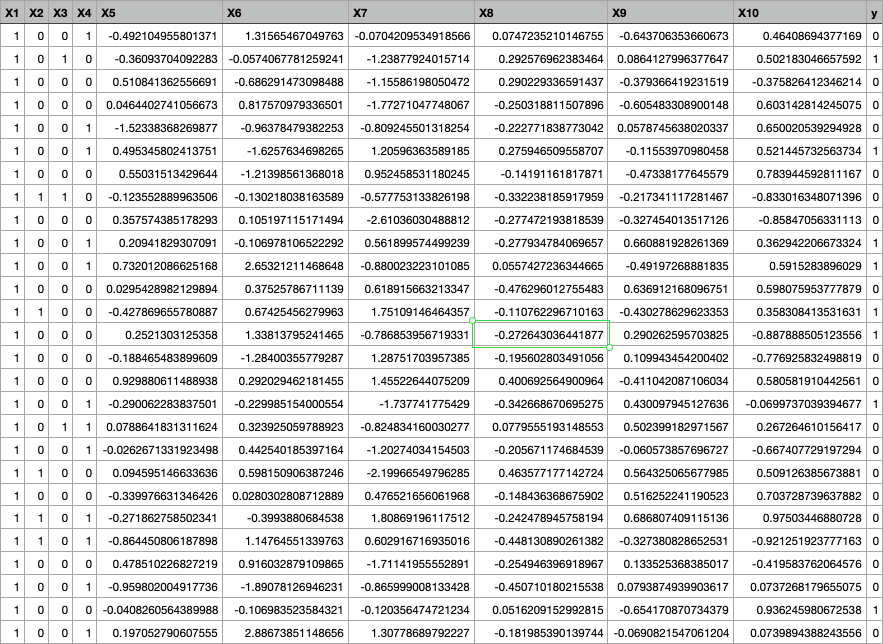
\includegraphics[scale=0.55]{data_screenshot.jpg}
\end{figure*}
\newpage
\section*{Notations}
\begin{itemize}
	\item $X_{1,2,3,4}$ are independent categorical data
	\item $X_{5,\dots, 10}$ are independent continuous data
	\item $y$ is the outcome\
	\item $sen$ denotes the sensitivity
	\item $sp$ denotes the specificity
	\item $N$ is the sample size\
	\item $\epsilon$ is the random error follows $\mathcal N(0,1)$
	\item $\beta$ is the true variables in $\mathds R^{10}$
	\item $\Sigma$ is the covariance matrix of trivariate normal distribution, defined as identity matrix $I_3$
	\item $\mu$ is the random effect in $\mathds R_3$ space
\end{itemize}
\section*{Data generation process}
First, let's define the true sensitivity and specificity as
\[
sen = 0.6\quad\text{and}\quad sp = 0.9
\]
and $\beta=(-1.5,0.1,-0.5,-0.3,0.4,-0.2,-0.25,0.35,-0.1,0.5)$.

Also define $X_1=\mathbb{1}_N$ as the intercept, and $X_2,X_3,X_4$ are generated with Bernoulli distribution \eqref{eq1} with  probability $p=0.1,0.3,0.5$ respectively.
\begin{equation}\label{eq1}
	f(X_i ; p)=\left\{\begin{array}{ll}
p & \text { if } X_i=1 \\
q=1-p & \text { if } X_i=0
\end{array}\right.
\end{equation}
then $X_5, X_6, X_7$ are generated from normal distributions $\mathcal N(0,0.5),\mathcal N(0,1),\mathcal N(0,1.5)$ respectively. Lastly, $X_8, X_9, X_{10}$ are generate from uniform distributions $\mathcal U(-0.5,0.5)$, $\mathcal U(-0.7,0.7)$, $\mathcal U(-1,1)$ respectively.

We generate the random effect $\mu$ using trivariate normal distribution 
\begin{equation}
	\mathcal N_3\bigbrac{\bigbrac{\begin{array}{ccc}
		0\\0\\0\\
	\end{array}}, \Sigma}, \quad\Sigma=I_3
\end{equation}
and with the settings, we can deduce the log-odds ratio with following formula
\begin{equation}
\log(\pi)=f(X\beta +\mu_1+\epsilon)
\end{equation}
where $f$ is the sigmoid function defined as
\begin{equation}
f(x)=\dfrac{e^x}{1+e^x}
\end{equation}

Now, we generate the outcomes $y$ for each sample with Bernoulli distribution \eqref{eq1} where the log-odds ratio served as the probability $p$.
Also, the sensitivity and specificity can be calculated with Binomial distribution with probability $sen+\mu_2$ and $sp+\mu_3$.

























\end{document}